\documentclass[11pt,a4paper]{article}
\usepackage[margin=1in]{geometry}
\usepackage{booktabs}
\usepackage{graphicx}
\usepackage{xcolor}
\usepackage{hyperref}
\usepackage{parskip}
\definecolor{spotter}{HTML}{064A56}
\hypersetup{colorlinks=true,linkcolor=spotter,urlcolor=spotter}
\title{\textcolor{spotter}{Spotter Freight Rate Prediction}}
\author{Machine Learning Assessment}
\date{November 2026}
\begin{document}
\maketitle

\section*{Objective}
The objective is to predict \texttt{posted\_rate} for 12,000 future loads.
The final submission was generated by refitting the selected model on all 48,000
labeled development rows.

\section*{Data and quality checks}
The development data covers 1 January--31 October 2025 and contains 48,000
rows. Training has 300 missing weights, 374 missing market-index values, and
292 negative weights. Validation has 165 missing weights and 249 missing
market-index values. There are no duplicate load IDs or non-positive distances.
Validation contains 8 unseen pickup cities, 8 unseen delivery cities, and 736
unseen routes. All observations were retained: missingness indicators and
training-fold median imputation handle missing values, while absolute weight
features preserve information from negative observations without inventing a
row-removal rule.

\section*{Feature engineering}
The pipeline creates route and route-equipment interactions, city/equipment
frequency features, haversine distance, geographic-distance ratio, route
direction, distance and weight transforms, distance-weight interactions,
market/quote interactions, missingness indicators, date components, and cyclic
seasonality. Frequency features are fitted inside each training fold only.
Categorical values use unknown-safe ordinal encoding. Scaling is applied to
Ridge and LinearSVR; tree and boosting models use unscaled features.

\section*{Validation methodology}
The latest 20\% of unique dates is an untouched final holdout: training and
tuning use 1 January--1 September, while the holdout is 2 September--31 October.
Model selection before that holdout uses four expanding validation windows, each
covering 28 complete dates. Every row from a date stays in the same partition.
This fixes the previous row-based \texttt{TimeSeriesSplit} issue and tests
multiple future monthly windows. The complete fold-level results are in
\texttt{reports/fold\_metrics.csv}.

\section*{Model comparison}
\begin{table}[h]
\centering
\small
\caption{Grouped chronological CV and untouched holdout results}
\begin{tabular}{lrrrrrr}
\toprule
Model & CV MAE & Latest MAE & Holdout MAE & RMSE & R-squared & MAPE (\%)\\
\midrule
MarketAdjustedLGBM & 99.76 & 103.59 & 103.15 & 633.96 & 0.8280 & 4.57\\
XGBRegressor & 103.20 & 106.17 & 108.15 & 639.57 & 0.8249 & 4.66\\
LGBMRegressor & 104.66 & 111.85 & 109.15 & 639.58 & 0.8249 & 4.69\\
CatBoostRegressor & 110.25 & 101.28 & 120.13 & 641.93 & 0.8237 & 5.37\\
LinearSVR & 141.64 & 127.80 & 155.33 & 649.90 & 0.8192 & 8.07\\
HistGradientBoosting & 160.49 & 138.21 & 133.03 & 644.56 & 0.8222 & 5.98\\
Ridge & 162.76 & 140.05 & 176.51 & 654.65 & 0.8166 & 10.48\\
ExtraTrees & 176.12 & 167.28 & 141.91 & 648.78 & 0.8199 & 6.24\\
DecisionTree & 217.16 & 218.03 & 198.38 & 700.07 & 0.7903 & 8.33\\
RandomForest & 234.09 & 192.68 & 186.59 & 676.44 & 0.8042 & 8.07\\
\bottomrule
\end{tabular}
\end{table}

Market-adjusted LightGBM was selected by chronological CV, not by repeated
holdout optimization. It achieved grouped-CV MAE 99.76 and holdout MAE 103.15,
while the closest alternatives were XGBoost at 108.15 and standard LightGBM at
109.15. Regularisation is explicit in the selected LightGBM configuration:
learning rate 0.03, 600 estimators, 31 leaves, 30 minimum child samples, and
L2 regularisation 5.

\section*{Extreme-error analysis}
There are 317 development observations above \$5/mile. They are spread across
all equipment types and dates, so no defensible single-category filter was
found. On the final holdout, 67 rows exceed \$5/mile: 44 Dry Van, 16 Reefer,
and 7 Flatbed. The median absolute error is 31.0, the 90th percentile is
118.0, the 95th percentile is 161.8, the 99th percentile is 1,606.2, and the
maximum is 16,241.7. The largest 1\% of absolute residuals contribute 97.4\%
of squared error. These observations are retained and exported in
\texttt{reports/residual\_analysis.csv} rather than capped without evidence.

\begin{figure}[h]
\centering
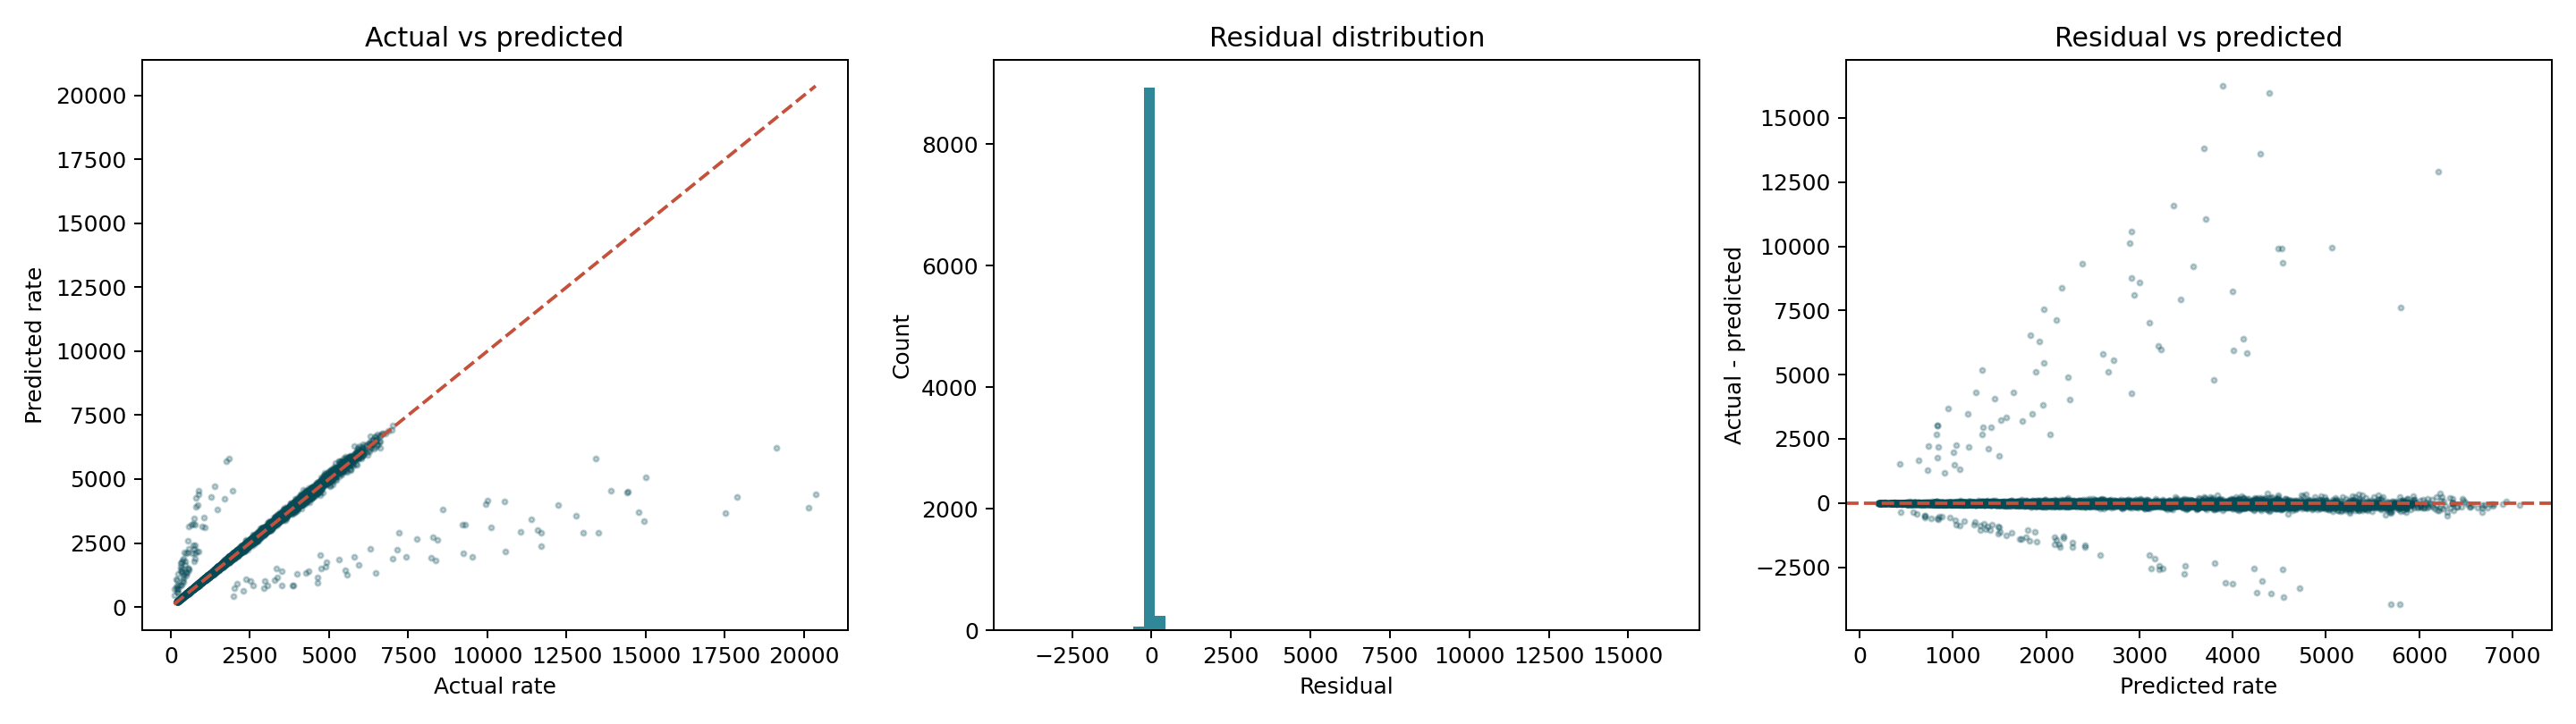
\includegraphics[width=\textwidth]{figures/residual_diagnostics.png}
\caption{Holdout actual versus predicted values and residual diagnostics.}
\end{figure}

\section*{Final outputs}
\texttt{validation\_predictions.csv} contains exactly two columns and 12,000
positive finite predictions in template order. \texttt{december\_predictions.csv}
contains 31 rows and leaves the supplied \texttt{december-chart-inputs.csv}
unchanged. The supplied \texttt{score.py} validates both files and generates
\texttt{figures/candidate\_december.png}.

\begin{figure}[h]
\centering
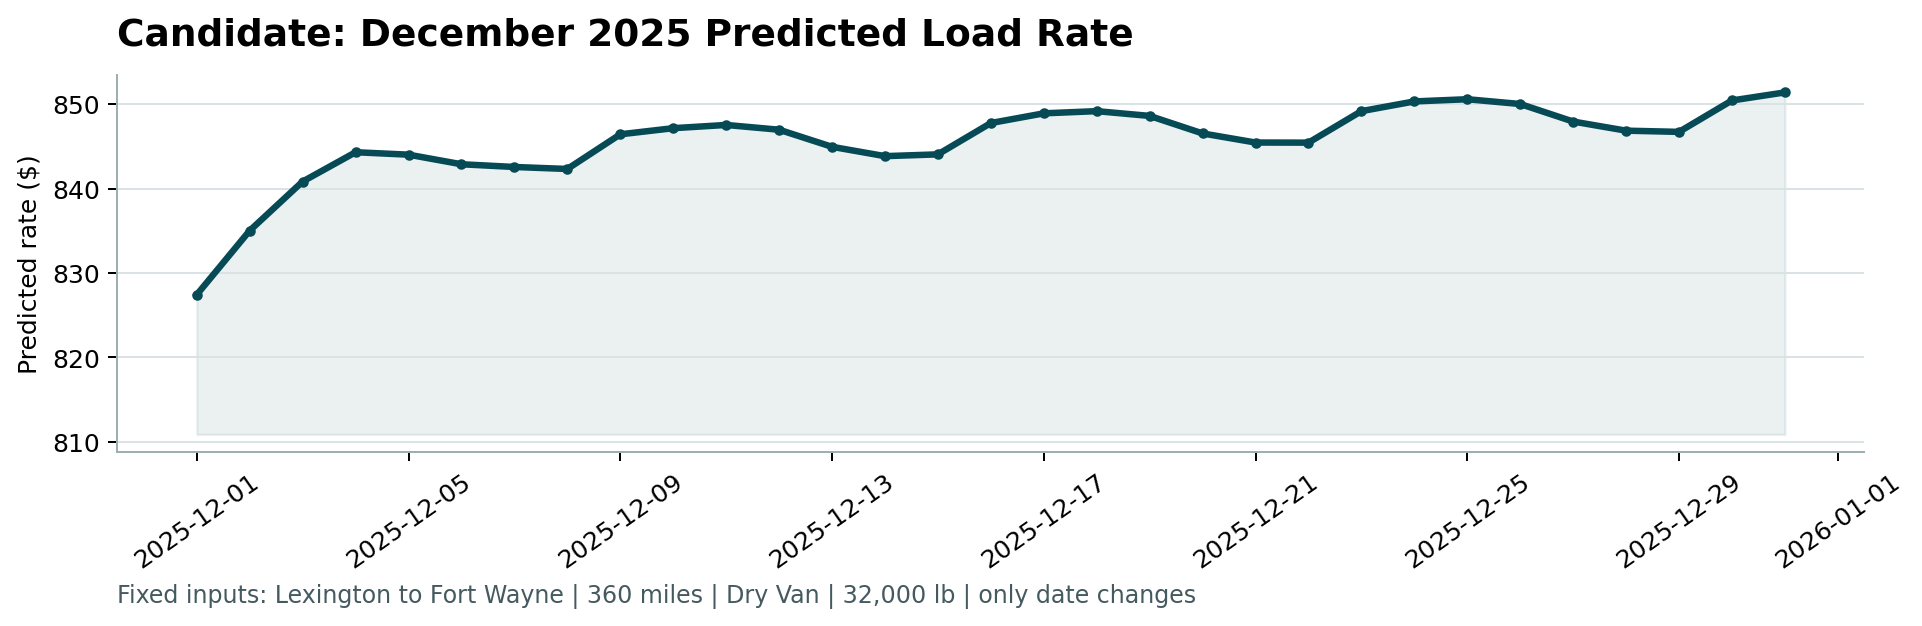
\includegraphics[width=\textwidth]{figures/candidate_december.png}
\caption{December 2025 prediction chart generated by the supplied scorer.}
\end{figure}

\section*{Reproduction}
\begin{verbatim}
python -m pip install -r requirements.txt
python src/train.py --data train-test.csv
python src/predict.py
python score.py --predictions validation_predictions.csv ^
  --december-predictions december_predictions.csv --output-dir reports/figures
\end{verbatim}

\end{document}
